\documentclass[12pt,a4paper,titlepage]{article}
\usepackage[utf8]{inputenc}
\usepackage{polski}
\usepackage{listings}
\usepackage{graphicx}
\usepackage{xcolor}
\usepackage{minted}
\usepackage{amsmath}
\usepackage{caption}
 
\setminted{
    linenos=true,
    autogobble,
    breaklines,
    frame=lines,
    framerule=1pt,
    framesep=10pt
}

\newenvironment{longlisting}{}{}

\makeatletter
\newcommand{\linia}{\rule{\linewidth}{0.4mm}}
\renewcommand{\maketitle}{\begin{titlepage}
    \vspace*{1cm}
    \begin{center}\small
    Politechnika Wrocławska\\
    Wydział Elektroniki\\
    Grafika Komputerowa i Komunikacja Człowiek-Komputer
    \end{center}
    \vspace{3cm}
    \noindent\linia
    \begin{center}
      \LARGE \textsc{\@title}
         \end{center}
     \linia
    \vspace{0.5cm}
    \begin{flushright}
    \begin{minipage}{7cm}
    \textit{\small Autor:}\\
    \normalsize \textsc{\@author} \par
    \end{minipage}
    \vspace{5cm}

     {\small czwartek, 17\textsuperscript{15}-20\textsuperscript{15} TN}\\
        mgr inż. Szymon Datko
     \end{flushright}
    \vspace*{\stretch{6}}
    \begin{center}
    \@date
    \end{center}
  \end{titlepage}%
}
\makeatother
\author{Justyna Skalska, 225942}
\title{Sprawozdanie nr 3\\
(OpenGL - interakcja z użytkownikiem)}

\begin{document}

\maketitle
\section{Omówienie tematu}
Naszym zadaniem na laboratoriach było stworzenie prostego programu wprowadzającego do interakcji z użytkownikiem z wykorzystaniem OpenGL wraz z rozszerzeniem GLUT. Główne zadanie polegało na sterowaniu ruchem  i położeniem obserwatora w przestrzeni 3D. Do sterowania służyła mysz, lewy przycisk odpowiadał za ruch wokół obiektu, a prawy za przybliżenie obserwatora. Równania punktów dla położenia obserwatora:

\begin{equation}
    \begin{split}
    & x_{s}(\Theta, \Phi) = R\cos{(\Theta)}\cos{(\Phi)} \\
    & y_{s}(\Theta, \Phi) = R\sin{(\Phi)} \\
    & z_{s}(\Theta, \Phi) = R\sin{(\Theta)}\cos{(\Phi)}
    \end{split}
    \quad\quad
    \begin{split}
        & 0 \le \Theta \le 2\pi \\
        & 0 \le \Phi   \le 2\pi
    \end{split}
\end{equation}
\newline\newline
Podczas wykonywania zadania dowiedziałam się także jak implementować rzut perspektywiczny.

\begin{figure}[H]
\centering
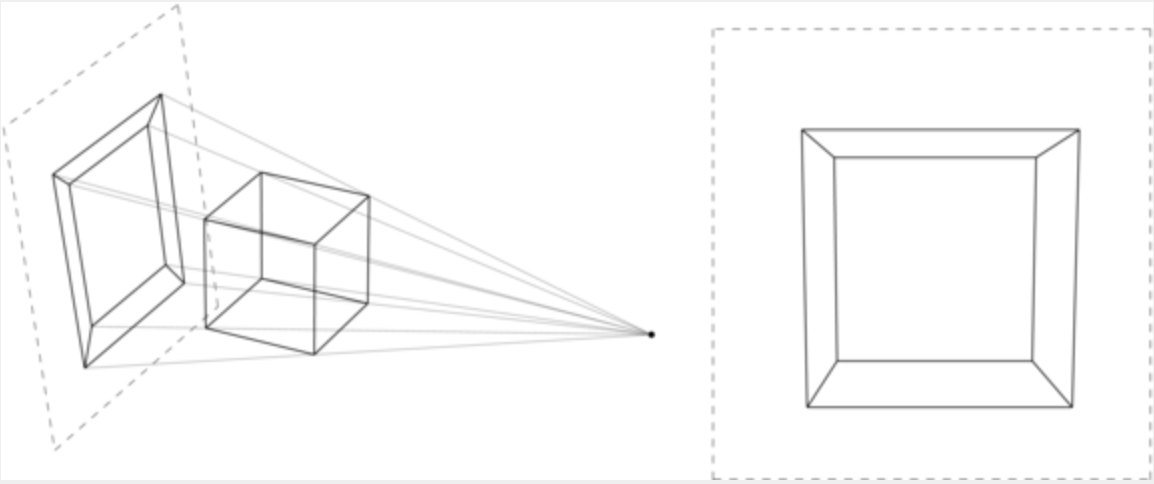
\includegraphics[width = 10cm]{images/perspektywa.png}
\caption{Rzutowanie perspektywiczne}
\label{fig:perspektywa}
\end{figure}

\section{Omówienie kodu}

\begin{listing}[H]
\caption{Zmienne globalne programu}
\begin{minted}{C++}
//pozycja obserwatora
static GLfloat viewer[] = { 0.0, 0.0, 10.0 };

// przybliżenie
static double R = 10.0;

// kąt obrotu obiektu
static GLfloat theta = 0.0;
static GLfloat phi = 0.0;

// przelicznik pikseli na stopnie
static GLfloat pix2angle;
static GLfloat piy2angle;

// stan klawiszy myszy 
// 0 - nie naciśnięto żadnego klawisza
// 1 - naciśnięty został lewy klawisz
// 2 - naciśnięty został prawy klawisz
static GLint status = 0;
							   
// poprzednia pozycja kursora myszy
static int x_pos_old = 0; 
static int y_pos_old = 0;

// różnica pomiędzy pozycją bieżącą i poprzednią kursora myszy
static int delta_x = 0;
static int delta_y = 0;
\end{minted}
\end{listing}

\begin{listing}
\caption{Funkcja aktualizująca położenie obserwatora}
\begin{minted}{C++}
void updateViewerPosition(){
    viewer[0] = R * cos(theta) * cos(phi);
    viewer[1] = R * sin(phi);
    viewer[2] = R * sin(theta) * cos(phi);
}
\end{minted}
\end{listing}

\begin{listing}[H]
\caption{Funkcja modyfikująca polecania rysujące}
\begin{minted}{C++}
void RenderScene(void) {
    // czyszczenie okna aktualnym kolorem czyszczącym
    glClear(GL_COLOR_BUFFER_BIT | GL_DEPTH_BUFFER_BIT);
    
    // czyszczenie macierzy bieżącej
    glLoadIdentity();
    
    // zdefiniowanie położenia obserwatora
    updateViewerPosition();
    gluLookAt(viewer[0], viewer[1], viewer[2], 0.0, 0.0, 0.0, 0.0, cos(phi), 0.0);
    
    // Narysowanie osi przy pomocy funkcji zdefiniowanej powyżej
    Axes();

    // Ustawienie koloru rysowania na biały
    glColor3f(1.0f, 1.0f, 1.0f);
    // rysowanie jajka
    drawEgg(N);

    glFlush();
    // Przekazanie poleceń rysujących do wykonania
    glutSwapBuffers();
}
\end{minted}
\end{listing}

\begin{listing}[H]
\caption{Funkcja odczytująca dane z myszy}
\begin{minted}{C++}
void Mouse(int btn, int state, int x, int y) {
    if (btn == GLUT_LEFT_BUTTON && state == GLUT_DOWN) {
        // przypisanie aktualnie odczytanej pozycji kursora jako pozycji poprzedniej
        x_pos_old = x;
        y_pos_old = y;
        status = 1; // wciśnięty został lewy klawisz myszy
    } else if (btn == GLUT_RIGHT_BUTTON && state == GLUT_DOWN) {
        // przypisanie aktualnie odczytanej pozycji kursora jako pozycji poprzedniej
        y_pos_old = y;
        status = 2; // wciśnięty został lewy klawisz myszy
    } else {
        status = 0; // nie został wciśnięty żaden klawisz
    }
}
\end{minted}
\end{listing}

\begin{listing}[H]
\caption{Funkcja odczytująca ruch z myszy}
\begin{minted}{C++}
void Motion(GLsizei x, GLsizei y) {
    // obliczenie różnicy położenia kursora myszy
    delta_x = x - x_pos_old;
    delta_y = y - y_pos_old;

    // modyfikacja kąta obrotu o kat proporcjonalny
    if (status == 1) {
        theta += delta_x * pix2angle;
        if (theta >= 360.0) {
            theta = 0.0;
        }
        phi += delta_y * piy2angle;
        if (phi >= 360.0) {
            phi = 0.0;
        }
    } else if (status == 2) {
        R += delta_y * 0.1;
        if (R <= 10) {
            R = 10;
        }
        if (R >= 20) {
            R = 20;
        }
    }

    // podstawienie bieżącego położenia jako poprzednie
    x_pos_old = x;
    y_pos_old = y;
    // przerysowanie obrazu sceny
    glutPostRedisplay();
}
\end{minted}
\end{listing}

\begin{listing}[H]
\caption{Główna funkcja programu}
\begin{minted}{C++}
int main(int argc, char * argv[]) {
    // ... pominięty kod z instrukcji
    // ustawia funkcję zwrotną myszy odpowiedzialną za badanie stanu myszy
    glutMouseFunc(Mouse);
    // ustawia funkcję zwrotną odpowiedzialną za badanie ruchu myszy
    glutMotionFunc(Motion);
    // ... pominięty kod z instrukcji
}
\end{minted}
\end{listing}

\section{Rezultat prac}
Udało mi się wykonać wszystkie podpunkty zadania. Kamera obracała się wokół obiektu, a naciśnięcie prawego przycisku myszy powodowało przybliżenie oraz oddalenie obserwatora względem obiektu. Dzięki temu można było oglądać jajo z każdej strony. Przybliżenie pozwalało dostrzec szczegóły obiektu.\\\\
Aplikacja pokazana na zdjęciach wykorzystuje jajko zbudowane z linii, aby lepiej było widać osie sceny względem, których porusza się obserwator.

\begin{figure}[H]
\centering
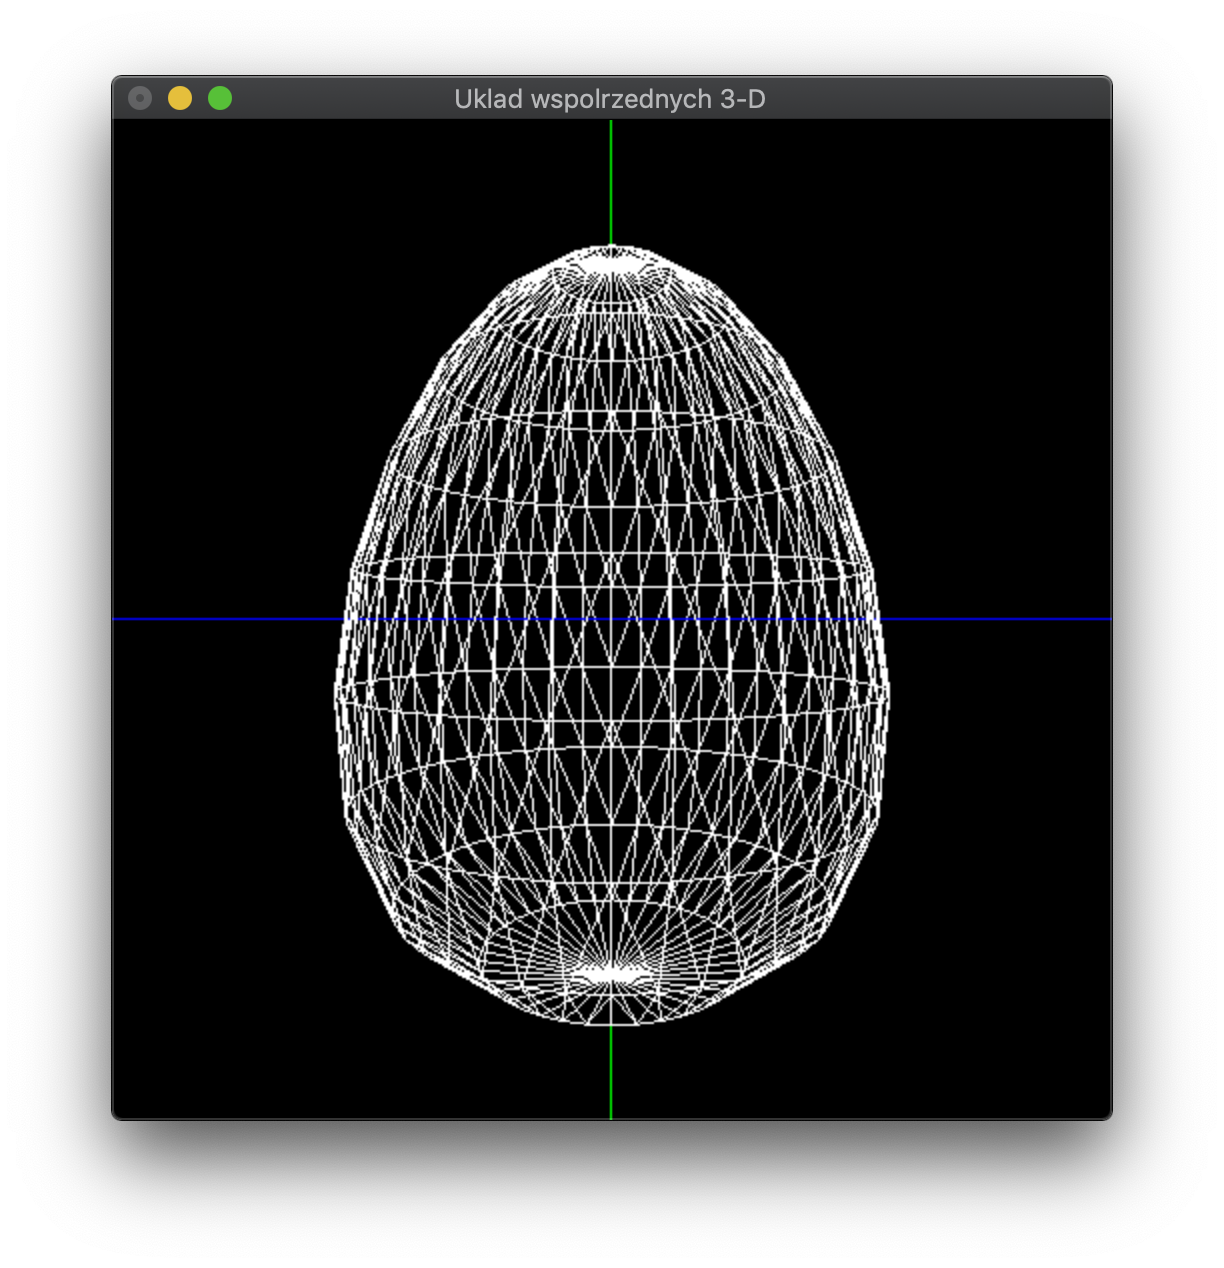
\includegraphics[width = 14cm]{images/initial.png}
\caption{Początkowa i najbliższa pozycja obserwatora}
\label{fig:egg_inital}
\end{figure}

\begin{figure}[H]
\centering
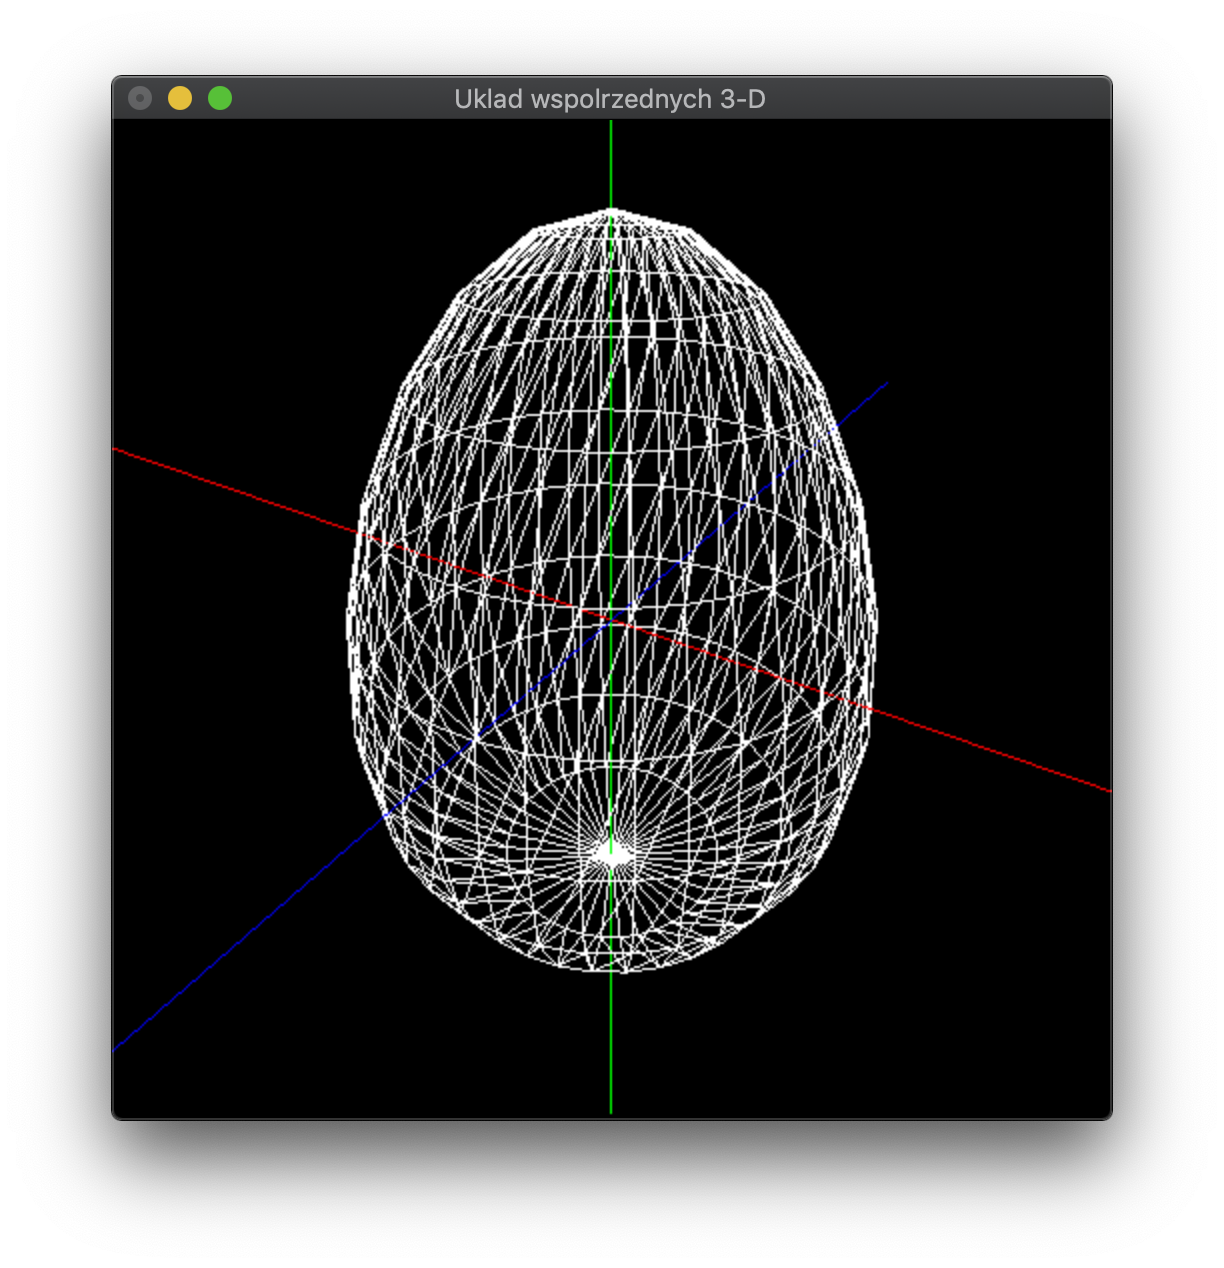
\includegraphics[width = 14cm]{images/rotated.png}
\caption{Obrócona pozycja obserwatora}
\label{fig:egg_rotated}
\end{figure}

\begin{figure}[H]
\centering
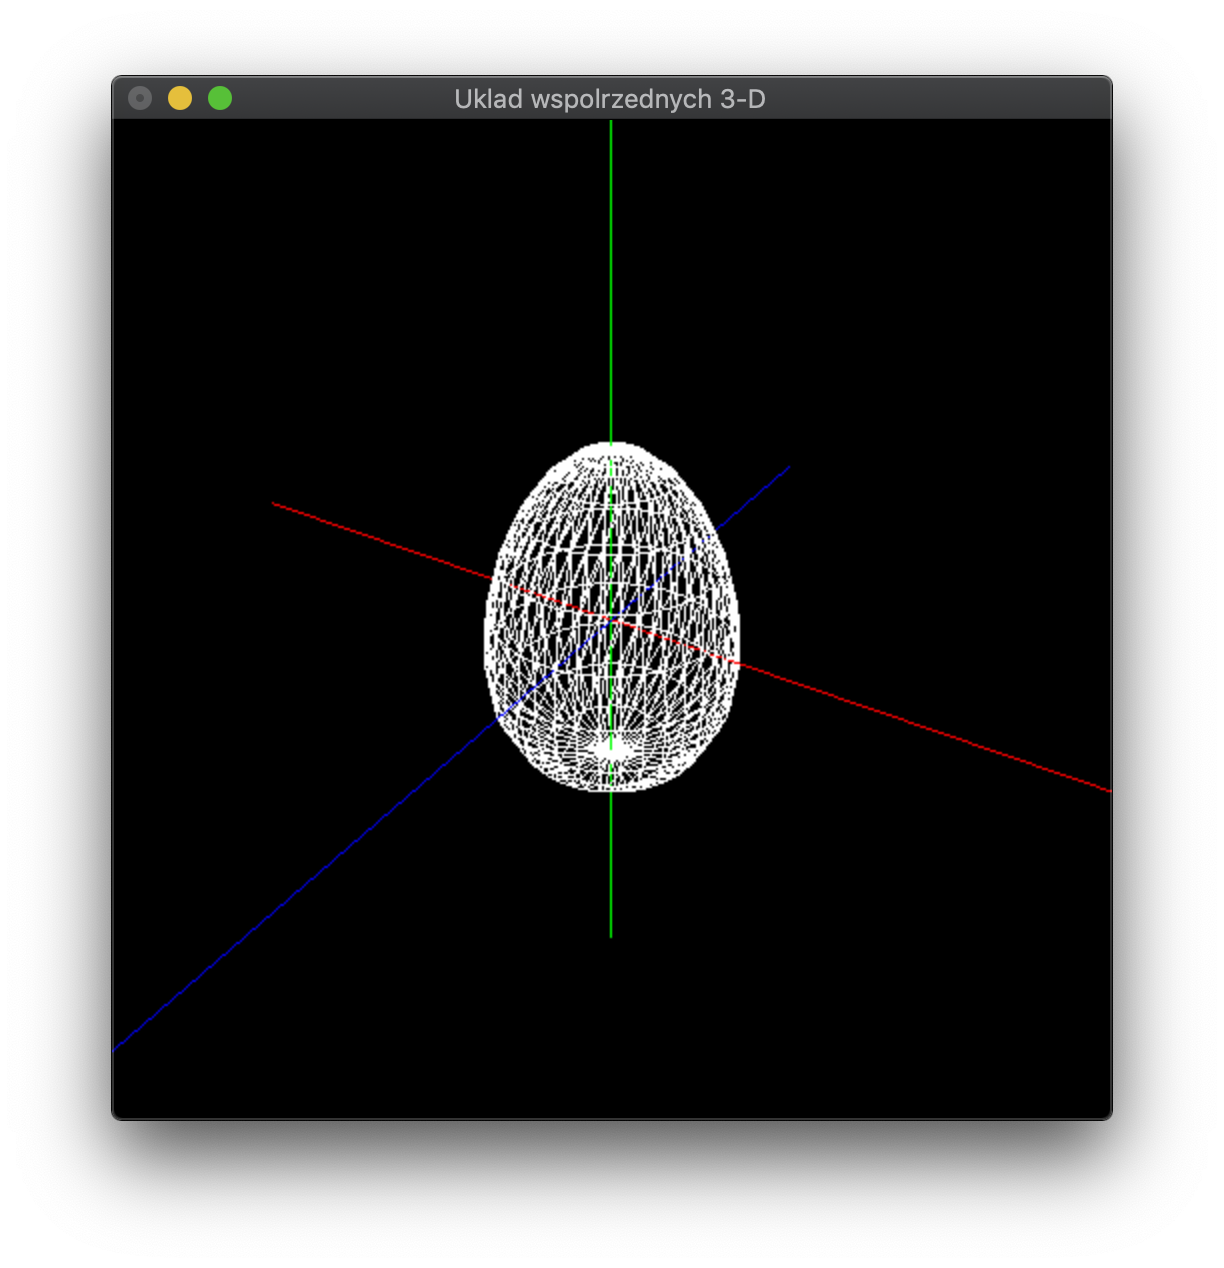
\includegraphics[width = 14cm]{images/zoomed_out.png}
\caption{Pozycja obserwatora oddalona od jajka o maksymalną odległość}
\label{fig:egg_zoomed_out}
\end{figure}

\end{document}
